
% 
% Annual Cognitive Science Conference
% Sample LaTeX Paper -- Proceedings Format
% 

% Original : Ashwin Ram (ashwin@cc.gatech.edu)       04/01/1994
% Modified : Johanna Moore (jmoore@cs.pitt.edu)      03/17/1995
% Modified : David Noelle (noelle@ucsd.edu)          03/15/1996
% Modified : Pat Langley (langley@cs.stanford.edu)   01/26/1997
% Latex2e corrections by Ramin Charles Nakisa        01/28/1997 
% Modified : Tina Eliassi-Rad (eliassi@cs.wisc.edu)  01/31/1998
% Modified : Trisha Yannuzzi (trisha@ircs.upenn.edu) 12/28/1999 (in process)
% Modified : Mary Ellen Foster (M.E.Foster@ed.ac.uk) 12/11/2000
% Modified : Ken Forbus                              01/23/2004
% Modified : Eli M. Silk (esilk@pitt.edu)            05/24/2005
% Modified : Niels Taatgen (taatgen@cmu.edu)         10/24/2006
% Modified : David Noelle (dnoelle@ucmerced.edu)     11/19/2014

%% Change ''letterpaper'' in the following line to ''a4paper'' if you must.

\documentclass[10pt,letterpaper]{article}

\usepackage{cogsci}
\usepackage{pslatex}
\usepackage{apacite}
\usepackage{amsmath,amssymb}
\usepackage{graphicx}
\usepackage{color}
\usepackage{url}
\usepackage{todonotes}
\usepackage{mathtools}
\usepackage{stmaryrd}
\usepackage{booktabs}
\usepackage{array}

\newcommand{\den}[2][]{
\(
\left\llbracket\;\text{#2}\;\right\rrbracket^{#1}
\)
}

%\newcommand{\url}[1]{$#1$}


\definecolor{Blue}{RGB}{0,0,255}
\newcommand{\jd}[1]{\textcolor{Blue}{[jd: #1]}}  
\definecolor{Red}{RGB}{255,0,0}
\newcommand{\red}[1]{\textcolor{Red}{#1}}
\definecolor{Green}{RGB}{10,200,100}
\newcommand{\ndg}[1]{\textcolor{Green}{[ndg: #1]}}
\definecolor{Red}{RGB}{255,0,0}
\newcommand{\caroline}[1]{\textcolor{Red}{#1}}


 \newcommand{\denote}[1]{\mbox{ $[\![ #1 ]\!]$}}


\newcommand{\subsubsubsection}[1]{{\em #1}}
\newcommand{\eref}[1]{(\ref{#1})}
\newcommand{\tableref}[1]{Table \ref{#1}}
\newcommand{\figref}[1]{Fig.~\ref{#1}}
\newcommand{\appref}[1]{Appendix \ref{#1}}
\newcommand{\sectionref}[1]{Section \ref{#1}}

\title{Learning to communicate about conceptual hierarchies}
%Animal, dog, or dalmatian? Contextual informativeness, utterance length and utterance frequency affect choice of referring expressions.

 
\author{{\large \bf Robert X.D. Hawkins, Michael Franke, Kenny Smith, Noah D.~Goodman} \\
  \{rxdh,ngoodman\}@stanford.edu\\
  Department of Psychology, Stanford University}

\begin{document}

\maketitle


\begin{abstract}
 In addition to several qualitative measures of differences in the lexical conventions that emerge, we introduce a model-based approach to infer participants' developing lexica throughout the game. 
\end{abstract}

\section{Introduction}

Natural languages provide speakers with remarkable flexibility in the labels they may use to refer to things (Brown, 1958; Cruse, 1977). In addition to the combinatorial explosion of modifiers afforded by compositionality (Winters, Kirby, \& Smith, 2014, Partee, 1995), we have a number of overlapping and nested terms in our lexicon. \emph{Fido}, \emph{Dalmatian}, \emph{dog}, and \emph{animal} can all reasonably be used to talk about the same entity at different levels of abstraction. How these overlapping meanings are learned, and why speakers choose different levels of specificity in different contexts, is increasingly well-understood \cite<e.g.>{XuTenenbaum07_WordLearningBayesian,GrafEtAl16_BasicLevel} but there remains a more fundamental question about the structure of our lexicon: how do abstractions become lexicalized in the first place? 

In this paper, we argue that just as communicative pressures for informativity lead to the lexicalization of specific terms when fine distinctions must be drawn, conceptual abstractions become lexicalized precisely when meaning is under-constrained by context. When the pragmatics of the context allow for ambiguity in the intended level of reference, adaptive users can get away with extending the term more broadly. 

This hypothesis is motivated by recent computational approaches to language evolution arguing that the lexical conventions of languages balance simplicity, or learnability, with the communicative needs of their users. This optimal expressivity hypothesis accounts well for the lexical distributions found in natural languages across semantic domains like color words and kinship categories \cite{RegierKempKay15_WordMeaningsEfficientCommunication}, as well as the compositional systems that emerge under iterated learning with communication in the lab \cite{WintersKirbySmith14_LanguagesAdapt, KirbyTamarizCornishSmith15_CompressionCommunication}.

While globally shared conventions of a language are shaped over the multi-generational timescales of cultural evolution, similar pressures may operate at the shorter timescales of dyadic interaction. In a matter of minutes, communication partners coordinate on efficient but informative local conventions for the task at hand (Clark \& Wilkes-Gibbs, 1986; Brennan \& Clark, 1996; Hawkins et al, 2017). The flexibility of these local cognitive mechanisms suggests that to understand the adaptiveness of languages to communicative constraints, it may be worth studying the adaptiveness of agents as they repeatedly interact. 
		 	
\section{Experiment 1: Hierarchical Reference}

To test this hypothesis, we conducted a repeated reference game in which pairs of participants interactively created an artificial language to communicate with each other about objects in context (e.g. Winters, Kirby, \& Smith, 2014; Galantucci \& Garrod, 2011). This paradigm allows us to fix a set of stimuli in a conceptual hierarchy and manipulate the communicative constraints of context across repeated interaction.

\begin{figure*}[t]
\begin{center}
{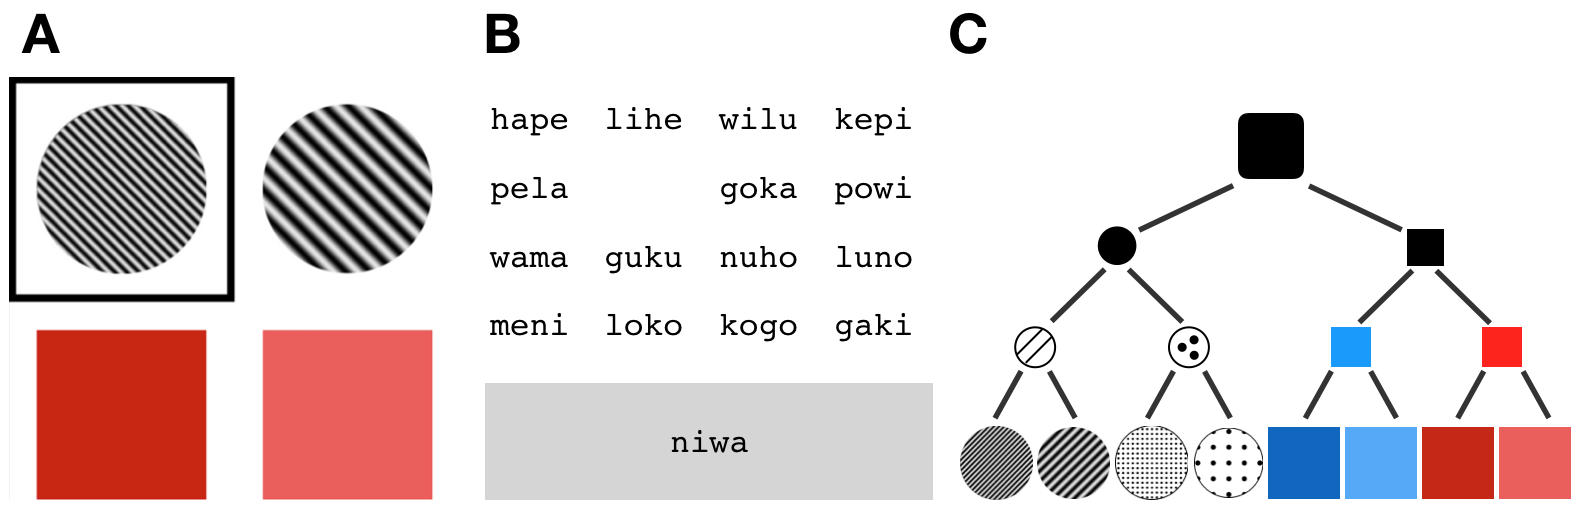
\includegraphics[scale=.64]{fig.png}}
{\caption{{\footnotesize (A) Example array of elements the matcher must choose from. The target is highlighted for the speaker with a black square. In this \emph{subordinate-required} trial there is a distractor at the same intermediate level (striped circle) as the target, so using any abstract label would be insufficient. (B) Drag-and-drop chat box interface. (C) Hierarchical organization of stimuli, with shape at the top-level and color/texture at intermediate levels.  \label{exp}}}}
\end{center}
\end{figure*}

\subsection{Methods}

\subsubsection{Participants}

We recruited 240 \todo[inline]{TODO: Update number}participants from Amazon Mechanical Turk to play an interactive, multi-player game using the framework described in \cite{Hawkins15_RealTimeWebExperiments}. Pairs were randomly assigned to one of three different conditions, yielding approximately $n=40$ games per condition.

\subsubsection{Stimuli}

The objects that served as referents were designed to cluster in a fixed three-level hierarchy with shape at the top-most level, and color/texture at the intermediate levels (see Fig. 1C). Each communicative context contained four objects. Distractors could differ from the target at various level of the hierarchy, creating different types of contexts defined by the finest distinction that had to be drawn. We focus on two: \emph{subordinate-neighbor} trials, where the closest distractor belongs to the same subordinate category (e.g. a lighter shade of blue square; see Fig. 1A), and \emph{intermediate-neighbor} trials, where the closest distractor belongs to the same intermediate category (e.g. red square instead of blue square). 

\subsubsection{Procedure}

Participants were paired over the web and placed in a shared environment containing a grid of four objects (Fig. 1A) and a `chatbox' to send messages from a randomly generated vocabulary of sixteen words (Fig. 1B). On each of 96 trials, one player -- the `speaker' -- was privately shown a highlighted target object and allowed to send a single word to communicate the identity of this object to their partner, who subsequently made a selection from the array. Players swapped roles each round and were rewarded with bonus payment when the listener successfully chose the intended object.

Critically, we manipulated the statistics of the context in a between-subjects design to test the effect of communicative relevance on lexicalization. In the \emph{pure subordinate} condition, all trials had a subordinate-neighbor context; in the \emph{pure intermediate} condition, all trials had a intermediate-neighbor context; in the \emph{mixed} condition, these two contexts were equally likely, thus providing more diversity in the relevant distinctions that must be drawn. 

In addition to behavioral responses collected over the course of the game, we designed a post-test to explicitly probe players' final lexica. For each word, we asked players to select all objects that word can refer to, and for each object, we asked players to select all words that can refer to it. These measures allow us to distinguish between subordinate terms that apply to only one element and abstract terms that apply to all elements belonging to an intermediate level of the hierarchy: striped circles, for example.

\subsection{Behavioral Results}

\subsubsection{People successfully learn to communicate}

Although participants began with no common basis for label meanings, most pairs were nonetheless able to coordinate on a successful communication system over repeated interaction. Accuracy improves significantly over the course of the experiment (b = 0.04, p < 0.001, random intercepts for games). These rates also differ across condition, with subordinate-necessary and uniform conditions unsurprisingly taking longer to converge [stat]. The time taken by the speaker to choose an utterance also decreases significantly over the course of the game [stat].

Still, the accuracy distribution was multi-modal: a subpopulation was still at chance (25\%) in the fourth quarter. For the subsequent analyses, we excluded all game with accuracy below 50\%.

\subsubsection{Context affects lexicon size}

We predicted that in contexts where speakers were not often required to draw fine distinctions at low levels of the conceptual hierarchy, they would instead develop abstract terms applying to everything below a particular node. One measure of the effect of to lexicon size: the more constraining context

\subsubsection{Context affects lexicon content}

We counted the relative number of subordinate-level terms and abstract terms in the post-test and found that the likelihood of lexicalizing abstractions differed significantly across conditions; in particular, the uniform condition was more likely to give rise to lexica in which multiple levels of reference coexist. 

\subsection{Model-based Results}

\subsubsection{Inferring participant's lexica over time}

How does the speaker's lexicon develop over the course of the game? We begin by analyzing this progression at a purely statistical level, without assuming any learning mechanisms in the mind of the agent. That is, we assume that on any given round, the speaker is using some fixed lexicon, and we invert a model of a pragmatic speaker to infer what that lexicon is. The goal of this is to (1) validate the post-test measures, (2) look at the time-course of basic-level vs. subordinate-level terms, (3) measure convergence, e.g. lexica changing less from round to round as game goes on? (4) measure path-dependence, e.g. how 

\section{Discussion}

This suggests that pragmatic pressures for informativity in a diversity of communicative contexts is instrumental for the lexicalization of hierarchical reference systems. Our separate minds may organize the world into meaningful conceptual hierarchies but our shared language only evolves to reflect this structure when it is communicatively relevant. 

What is the relationship between our concepts and words? While our individual mental representations of taxonomies are adaptive to the natural perceptual structure of the world (Rosch et al, 1976; Mervis \& Rosch ,1981; Murphy \& Smith, 1982), it is far from inevitable that all levels of these conceptual hierarchies become conventionalized as lexical items. There are many perfectly natural meanings that are not represented by distinct words in the English language: for instance, we do not have words for each individual tree in our yards, or for abstract but ad-hoc concepts like things to sell at a garage sale (Barsalou, 1983). Indeed, English speakers are often fascinated by difficult to express concepts like ``hygge'' or ``tartle'' that are lexicalized as simple words in foreign languages.

Another clear functional advantage of having abstract terms in the lexicon is that they allow speakers to efficiently refer to large, potentially infinite, sets of things and make generalizations about categories, e.g. ``Dogs bark'' (Tessler \& Goodman, 2016). 

We showed how abstractions become lexicalized when participants were restricted to single-word utterances, but how does this trade off with compositionality?

% Also elaborates on Bayesian accounts of word learning to context (Xu & Tenenbaum, 2007).


\section{\bf Acknowledgments}
\small
This work was supported by ONR grant N00014-13-1-0788 and a James S. McDonnell Foundation Scholar Award to NDG. RXDH was supported by the Stanford Graduate Fellowship and the National Science Foundation Graduate Research Fellowship under Grant No. DGE-114747.

\begin{figure*}[t]
\begin{center}
{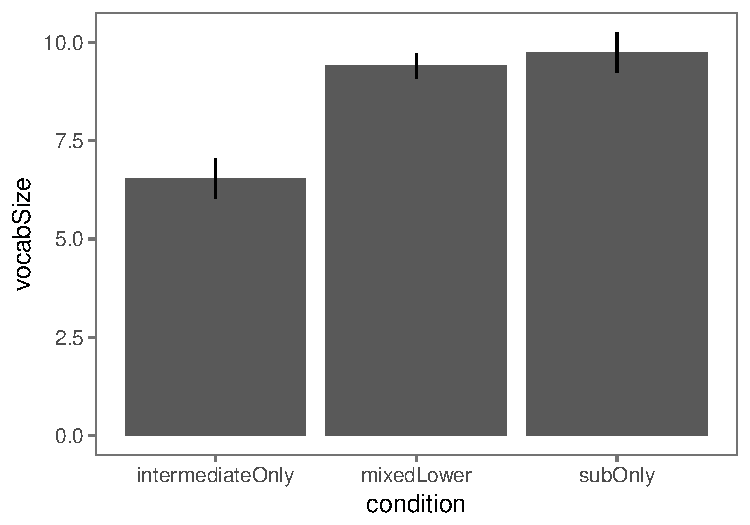
\includegraphics[scale=.64]{lexiconSize.pdf}}
{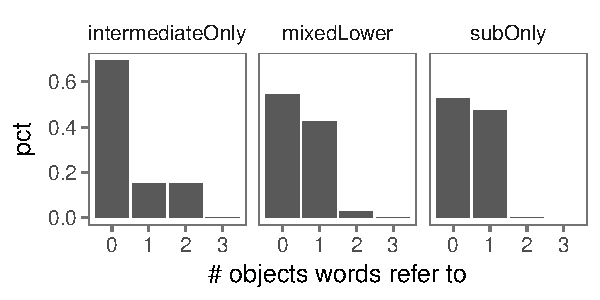
\includegraphics[scale=.64]{lexiconContent.pdf}}
{\caption{{\footnotesize (A)   \label{exp}}}}
\end{center}
\end{figure*}

\bibliographystyle{apacite}

\setlength{\bibleftmargin}{.125in}
\setlength{\bibindent}{-\bibleftmargin}

\bibliography{bibs}


\end{document}